
% Default to the notebook output style

    


% Inherit from the specified cell style.




    
\documentclass[11pt]{article}

    
    
    \usepackage[T1]{fontenc}
    % Nicer default font (+ math font) than Computer Modern for most use cases
    \usepackage{mathpazo}

    % Basic figure setup, for now with no caption control since it's done
    % automatically by Pandoc (which extracts ![](path) syntax from Markdown).
    \usepackage{graphicx}
    % We will generate all images so they have a width \maxwidth. This means
    % that they will get their normal width if they fit onto the page, but
    % are scaled down if they would overflow the margins.
    \makeatletter
    \def\maxwidth{\ifdim\Gin@nat@width>\linewidth\linewidth
    \else\Gin@nat@width\fi}
    \makeatother
    \let\Oldincludegraphics\includegraphics
    % Set max figure width to be 80% of text width, for now hardcoded.
    \renewcommand{\includegraphics}[1]{\Oldincludegraphics[width=.8\maxwidth]{#1}}
    % Ensure that by default, figures have no caption (until we provide a
    % proper Figure object with a Caption API and a way to capture that
    % in the conversion process - todo).
    \usepackage{caption}
    \DeclareCaptionLabelFormat{nolabel}{}
    \captionsetup{labelformat=nolabel}

    \usepackage{adjustbox} % Used to constrain images to a maximum size 
    \usepackage{xcolor} % Allow colors to be defined
    \usepackage{enumerate} % Needed for markdown enumerations to work
    \usepackage{geometry} % Used to adjust the document margins
    \usepackage{amsmath} % Equations
    \usepackage{amssymb} % Equations
    \usepackage{textcomp} % defines textquotesingle
    % Hack from http://tex.stackexchange.com/a/47451/13684:
    \AtBeginDocument{%
        \def\PYZsq{\textquotesingle}% Upright quotes in Pygmentized code
    }
    \usepackage{upquote} % Upright quotes for verbatim code
    \usepackage{eurosym} % defines \euro
    \usepackage[mathletters]{ucs} % Extended unicode (utf-8) support
    \usepackage[utf8x]{inputenc} % Allow utf-8 characters in the tex document
    \usepackage{fancyvrb} % verbatim replacement that allows latex
    \usepackage{grffile} % extends the file name processing of package graphics 
                         % to support a larger range 
    % The hyperref package gives us a pdf with properly built
    % internal navigation ('pdf bookmarks' for the table of contents,
    % internal cross-reference links, web links for URLs, etc.)
    \usepackage{hyperref}
    \usepackage{longtable} % longtable support required by pandoc >1.10
    \usepackage{booktabs}  % table support for pandoc > 1.12.2
    \usepackage[inline]{enumitem} % IRkernel/repr support (it uses the enumerate* environment)
    \usepackage[normalem]{ulem} % ulem is needed to support strikethroughs (\sout)
                                % normalem makes italics be italics, not underlines
    

    
    
    % Colors for the hyperref package
    \definecolor{urlcolor}{rgb}{0,.145,.698}
    \definecolor{linkcolor}{rgb}{.71,0.21,0.01}
    \definecolor{citecolor}{rgb}{.12,.54,.11}

    % ANSI colors
    \definecolor{ansi-black}{HTML}{3E424D}
    \definecolor{ansi-black-intense}{HTML}{282C36}
    \definecolor{ansi-red}{HTML}{E75C58}
    \definecolor{ansi-red-intense}{HTML}{B22B31}
    \definecolor{ansi-green}{HTML}{00A250}
    \definecolor{ansi-green-intense}{HTML}{007427}
    \definecolor{ansi-yellow}{HTML}{DDB62B}
    \definecolor{ansi-yellow-intense}{HTML}{B27D12}
    \definecolor{ansi-blue}{HTML}{208FFB}
    \definecolor{ansi-blue-intense}{HTML}{0065CA}
    \definecolor{ansi-magenta}{HTML}{D160C4}
    \definecolor{ansi-magenta-intense}{HTML}{A03196}
    \definecolor{ansi-cyan}{HTML}{60C6C8}
    \definecolor{ansi-cyan-intense}{HTML}{258F8F}
    \definecolor{ansi-white}{HTML}{C5C1B4}
    \definecolor{ansi-white-intense}{HTML}{A1A6B2}

    % commands and environments needed by pandoc snippets
    % extracted from the output of `pandoc -s`
    \providecommand{\tightlist}{%
      \setlength{\itemsep}{0pt}\setlength{\parskip}{0pt}}
    \DefineVerbatimEnvironment{Highlighting}{Verbatim}{commandchars=\\\{\}}
    % Add ',fontsize=\small' for more characters per line
    \newenvironment{Shaded}{}{}
    \newcommand{\KeywordTok}[1]{\textcolor[rgb]{0.00,0.44,0.13}{\textbf{{#1}}}}
    \newcommand{\DataTypeTok}[1]{\textcolor[rgb]{0.56,0.13,0.00}{{#1}}}
    \newcommand{\DecValTok}[1]{\textcolor[rgb]{0.25,0.63,0.44}{{#1}}}
    \newcommand{\BaseNTok}[1]{\textcolor[rgb]{0.25,0.63,0.44}{{#1}}}
    \newcommand{\FloatTok}[1]{\textcolor[rgb]{0.25,0.63,0.44}{{#1}}}
    \newcommand{\CharTok}[1]{\textcolor[rgb]{0.25,0.44,0.63}{{#1}}}
    \newcommand{\StringTok}[1]{\textcolor[rgb]{0.25,0.44,0.63}{{#1}}}
    \newcommand{\CommentTok}[1]{\textcolor[rgb]{0.38,0.63,0.69}{\textit{{#1}}}}
    \newcommand{\OtherTok}[1]{\textcolor[rgb]{0.00,0.44,0.13}{{#1}}}
    \newcommand{\AlertTok}[1]{\textcolor[rgb]{1.00,0.00,0.00}{\textbf{{#1}}}}
    \newcommand{\FunctionTok}[1]{\textcolor[rgb]{0.02,0.16,0.49}{{#1}}}
    \newcommand{\RegionMarkerTok}[1]{{#1}}
    \newcommand{\ErrorTok}[1]{\textcolor[rgb]{1.00,0.00,0.00}{\textbf{{#1}}}}
    \newcommand{\NormalTok}[1]{{#1}}
    
    % Additional commands for more recent versions of Pandoc
    \newcommand{\ConstantTok}[1]{\textcolor[rgb]{0.53,0.00,0.00}{{#1}}}
    \newcommand{\SpecialCharTok}[1]{\textcolor[rgb]{0.25,0.44,0.63}{{#1}}}
    \newcommand{\VerbatimStringTok}[1]{\textcolor[rgb]{0.25,0.44,0.63}{{#1}}}
    \newcommand{\SpecialStringTok}[1]{\textcolor[rgb]{0.73,0.40,0.53}{{#1}}}
    \newcommand{\ImportTok}[1]{{#1}}
    \newcommand{\DocumentationTok}[1]{\textcolor[rgb]{0.73,0.13,0.13}{\textit{{#1}}}}
    \newcommand{\AnnotationTok}[1]{\textcolor[rgb]{0.38,0.63,0.69}{\textbf{\textit{{#1}}}}}
    \newcommand{\CommentVarTok}[1]{\textcolor[rgb]{0.38,0.63,0.69}{\textbf{\textit{{#1}}}}}
    \newcommand{\VariableTok}[1]{\textcolor[rgb]{0.10,0.09,0.49}{{#1}}}
    \newcommand{\ControlFlowTok}[1]{\textcolor[rgb]{0.00,0.44,0.13}{\textbf{{#1}}}}
    \newcommand{\OperatorTok}[1]{\textcolor[rgb]{0.40,0.40,0.40}{{#1}}}
    \newcommand{\BuiltInTok}[1]{{#1}}
    \newcommand{\ExtensionTok}[1]{{#1}}
    \newcommand{\PreprocessorTok}[1]{\textcolor[rgb]{0.74,0.48,0.00}{{#1}}}
    \newcommand{\AttributeTok}[1]{\textcolor[rgb]{0.49,0.56,0.16}{{#1}}}
    \newcommand{\InformationTok}[1]{\textcolor[rgb]{0.38,0.63,0.69}{\textbf{\textit{{#1}}}}}
    \newcommand{\WarningTok}[1]{\textcolor[rgb]{0.38,0.63,0.69}{\textbf{\textit{{#1}}}}}
    
    
    % Define a nice break command that doesn't care if a line doesn't already
    % exist.
    \def\br{\hspace*{\fill} \\* }
    % Math Jax compatability definitions
    \def\gt{>}
    \def\lt{<}
    % Document parameters
    \title{Oracle\_Click\_Analytics}
    
    
    

    % Pygments definitions
    
\makeatletter
\def\PY@reset{\let\PY@it=\relax \let\PY@bf=\relax%
    \let\PY@ul=\relax \let\PY@tc=\relax%
    \let\PY@bc=\relax \let\PY@ff=\relax}
\def\PY@tok#1{\csname PY@tok@#1\endcsname}
\def\PY@toks#1+{\ifx\relax#1\empty\else%
    \PY@tok{#1}\expandafter\PY@toks\fi}
\def\PY@do#1{\PY@bc{\PY@tc{\PY@ul{%
    \PY@it{\PY@bf{\PY@ff{#1}}}}}}}
\def\PY#1#2{\PY@reset\PY@toks#1+\relax+\PY@do{#2}}

\expandafter\def\csname PY@tok@w\endcsname{\def\PY@tc##1{\textcolor[rgb]{0.73,0.73,0.73}{##1}}}
\expandafter\def\csname PY@tok@c\endcsname{\let\PY@it=\textit\def\PY@tc##1{\textcolor[rgb]{0.25,0.50,0.50}{##1}}}
\expandafter\def\csname PY@tok@cp\endcsname{\def\PY@tc##1{\textcolor[rgb]{0.74,0.48,0.00}{##1}}}
\expandafter\def\csname PY@tok@k\endcsname{\let\PY@bf=\textbf\def\PY@tc##1{\textcolor[rgb]{0.00,0.50,0.00}{##1}}}
\expandafter\def\csname PY@tok@kp\endcsname{\def\PY@tc##1{\textcolor[rgb]{0.00,0.50,0.00}{##1}}}
\expandafter\def\csname PY@tok@kt\endcsname{\def\PY@tc##1{\textcolor[rgb]{0.69,0.00,0.25}{##1}}}
\expandafter\def\csname PY@tok@o\endcsname{\def\PY@tc##1{\textcolor[rgb]{0.40,0.40,0.40}{##1}}}
\expandafter\def\csname PY@tok@ow\endcsname{\let\PY@bf=\textbf\def\PY@tc##1{\textcolor[rgb]{0.67,0.13,1.00}{##1}}}
\expandafter\def\csname PY@tok@nb\endcsname{\def\PY@tc##1{\textcolor[rgb]{0.00,0.50,0.00}{##1}}}
\expandafter\def\csname PY@tok@nf\endcsname{\def\PY@tc##1{\textcolor[rgb]{0.00,0.00,1.00}{##1}}}
\expandafter\def\csname PY@tok@nc\endcsname{\let\PY@bf=\textbf\def\PY@tc##1{\textcolor[rgb]{0.00,0.00,1.00}{##1}}}
\expandafter\def\csname PY@tok@nn\endcsname{\let\PY@bf=\textbf\def\PY@tc##1{\textcolor[rgb]{0.00,0.00,1.00}{##1}}}
\expandafter\def\csname PY@tok@ne\endcsname{\let\PY@bf=\textbf\def\PY@tc##1{\textcolor[rgb]{0.82,0.25,0.23}{##1}}}
\expandafter\def\csname PY@tok@nv\endcsname{\def\PY@tc##1{\textcolor[rgb]{0.10,0.09,0.49}{##1}}}
\expandafter\def\csname PY@tok@no\endcsname{\def\PY@tc##1{\textcolor[rgb]{0.53,0.00,0.00}{##1}}}
\expandafter\def\csname PY@tok@nl\endcsname{\def\PY@tc##1{\textcolor[rgb]{0.63,0.63,0.00}{##1}}}
\expandafter\def\csname PY@tok@ni\endcsname{\let\PY@bf=\textbf\def\PY@tc##1{\textcolor[rgb]{0.60,0.60,0.60}{##1}}}
\expandafter\def\csname PY@tok@na\endcsname{\def\PY@tc##1{\textcolor[rgb]{0.49,0.56,0.16}{##1}}}
\expandafter\def\csname PY@tok@nt\endcsname{\let\PY@bf=\textbf\def\PY@tc##1{\textcolor[rgb]{0.00,0.50,0.00}{##1}}}
\expandafter\def\csname PY@tok@nd\endcsname{\def\PY@tc##1{\textcolor[rgb]{0.67,0.13,1.00}{##1}}}
\expandafter\def\csname PY@tok@s\endcsname{\def\PY@tc##1{\textcolor[rgb]{0.73,0.13,0.13}{##1}}}
\expandafter\def\csname PY@tok@sd\endcsname{\let\PY@it=\textit\def\PY@tc##1{\textcolor[rgb]{0.73,0.13,0.13}{##1}}}
\expandafter\def\csname PY@tok@si\endcsname{\let\PY@bf=\textbf\def\PY@tc##1{\textcolor[rgb]{0.73,0.40,0.53}{##1}}}
\expandafter\def\csname PY@tok@se\endcsname{\let\PY@bf=\textbf\def\PY@tc##1{\textcolor[rgb]{0.73,0.40,0.13}{##1}}}
\expandafter\def\csname PY@tok@sr\endcsname{\def\PY@tc##1{\textcolor[rgb]{0.73,0.40,0.53}{##1}}}
\expandafter\def\csname PY@tok@ss\endcsname{\def\PY@tc##1{\textcolor[rgb]{0.10,0.09,0.49}{##1}}}
\expandafter\def\csname PY@tok@sx\endcsname{\def\PY@tc##1{\textcolor[rgb]{0.00,0.50,0.00}{##1}}}
\expandafter\def\csname PY@tok@m\endcsname{\def\PY@tc##1{\textcolor[rgb]{0.40,0.40,0.40}{##1}}}
\expandafter\def\csname PY@tok@gh\endcsname{\let\PY@bf=\textbf\def\PY@tc##1{\textcolor[rgb]{0.00,0.00,0.50}{##1}}}
\expandafter\def\csname PY@tok@gu\endcsname{\let\PY@bf=\textbf\def\PY@tc##1{\textcolor[rgb]{0.50,0.00,0.50}{##1}}}
\expandafter\def\csname PY@tok@gd\endcsname{\def\PY@tc##1{\textcolor[rgb]{0.63,0.00,0.00}{##1}}}
\expandafter\def\csname PY@tok@gi\endcsname{\def\PY@tc##1{\textcolor[rgb]{0.00,0.63,0.00}{##1}}}
\expandafter\def\csname PY@tok@gr\endcsname{\def\PY@tc##1{\textcolor[rgb]{1.00,0.00,0.00}{##1}}}
\expandafter\def\csname PY@tok@ge\endcsname{\let\PY@it=\textit}
\expandafter\def\csname PY@tok@gs\endcsname{\let\PY@bf=\textbf}
\expandafter\def\csname PY@tok@gp\endcsname{\let\PY@bf=\textbf\def\PY@tc##1{\textcolor[rgb]{0.00,0.00,0.50}{##1}}}
\expandafter\def\csname PY@tok@go\endcsname{\def\PY@tc##1{\textcolor[rgb]{0.53,0.53,0.53}{##1}}}
\expandafter\def\csname PY@tok@gt\endcsname{\def\PY@tc##1{\textcolor[rgb]{0.00,0.27,0.87}{##1}}}
\expandafter\def\csname PY@tok@err\endcsname{\def\PY@bc##1{\setlength{\fboxsep}{0pt}\fcolorbox[rgb]{1.00,0.00,0.00}{1,1,1}{\strut ##1}}}
\expandafter\def\csname PY@tok@kc\endcsname{\let\PY@bf=\textbf\def\PY@tc##1{\textcolor[rgb]{0.00,0.50,0.00}{##1}}}
\expandafter\def\csname PY@tok@kd\endcsname{\let\PY@bf=\textbf\def\PY@tc##1{\textcolor[rgb]{0.00,0.50,0.00}{##1}}}
\expandafter\def\csname PY@tok@kn\endcsname{\let\PY@bf=\textbf\def\PY@tc##1{\textcolor[rgb]{0.00,0.50,0.00}{##1}}}
\expandafter\def\csname PY@tok@kr\endcsname{\let\PY@bf=\textbf\def\PY@tc##1{\textcolor[rgb]{0.00,0.50,0.00}{##1}}}
\expandafter\def\csname PY@tok@bp\endcsname{\def\PY@tc##1{\textcolor[rgb]{0.00,0.50,0.00}{##1}}}
\expandafter\def\csname PY@tok@fm\endcsname{\def\PY@tc##1{\textcolor[rgb]{0.00,0.00,1.00}{##1}}}
\expandafter\def\csname PY@tok@vc\endcsname{\def\PY@tc##1{\textcolor[rgb]{0.10,0.09,0.49}{##1}}}
\expandafter\def\csname PY@tok@vg\endcsname{\def\PY@tc##1{\textcolor[rgb]{0.10,0.09,0.49}{##1}}}
\expandafter\def\csname PY@tok@vi\endcsname{\def\PY@tc##1{\textcolor[rgb]{0.10,0.09,0.49}{##1}}}
\expandafter\def\csname PY@tok@vm\endcsname{\def\PY@tc##1{\textcolor[rgb]{0.10,0.09,0.49}{##1}}}
\expandafter\def\csname PY@tok@sa\endcsname{\def\PY@tc##1{\textcolor[rgb]{0.73,0.13,0.13}{##1}}}
\expandafter\def\csname PY@tok@sb\endcsname{\def\PY@tc##1{\textcolor[rgb]{0.73,0.13,0.13}{##1}}}
\expandafter\def\csname PY@tok@sc\endcsname{\def\PY@tc##1{\textcolor[rgb]{0.73,0.13,0.13}{##1}}}
\expandafter\def\csname PY@tok@dl\endcsname{\def\PY@tc##1{\textcolor[rgb]{0.73,0.13,0.13}{##1}}}
\expandafter\def\csname PY@tok@s2\endcsname{\def\PY@tc##1{\textcolor[rgb]{0.73,0.13,0.13}{##1}}}
\expandafter\def\csname PY@tok@sh\endcsname{\def\PY@tc##1{\textcolor[rgb]{0.73,0.13,0.13}{##1}}}
\expandafter\def\csname PY@tok@s1\endcsname{\def\PY@tc##1{\textcolor[rgb]{0.73,0.13,0.13}{##1}}}
\expandafter\def\csname PY@tok@mb\endcsname{\def\PY@tc##1{\textcolor[rgb]{0.40,0.40,0.40}{##1}}}
\expandafter\def\csname PY@tok@mf\endcsname{\def\PY@tc##1{\textcolor[rgb]{0.40,0.40,0.40}{##1}}}
\expandafter\def\csname PY@tok@mh\endcsname{\def\PY@tc##1{\textcolor[rgb]{0.40,0.40,0.40}{##1}}}
\expandafter\def\csname PY@tok@mi\endcsname{\def\PY@tc##1{\textcolor[rgb]{0.40,0.40,0.40}{##1}}}
\expandafter\def\csname PY@tok@il\endcsname{\def\PY@tc##1{\textcolor[rgb]{0.40,0.40,0.40}{##1}}}
\expandafter\def\csname PY@tok@mo\endcsname{\def\PY@tc##1{\textcolor[rgb]{0.40,0.40,0.40}{##1}}}
\expandafter\def\csname PY@tok@ch\endcsname{\let\PY@it=\textit\def\PY@tc##1{\textcolor[rgb]{0.25,0.50,0.50}{##1}}}
\expandafter\def\csname PY@tok@cm\endcsname{\let\PY@it=\textit\def\PY@tc##1{\textcolor[rgb]{0.25,0.50,0.50}{##1}}}
\expandafter\def\csname PY@tok@cpf\endcsname{\let\PY@it=\textit\def\PY@tc##1{\textcolor[rgb]{0.25,0.50,0.50}{##1}}}
\expandafter\def\csname PY@tok@c1\endcsname{\let\PY@it=\textit\def\PY@tc##1{\textcolor[rgb]{0.25,0.50,0.50}{##1}}}
\expandafter\def\csname PY@tok@cs\endcsname{\let\PY@it=\textit\def\PY@tc##1{\textcolor[rgb]{0.25,0.50,0.50}{##1}}}

\def\PYZbs{\char`\\}
\def\PYZus{\char`\_}
\def\PYZob{\char`\{}
\def\PYZcb{\char`\}}
\def\PYZca{\char`\^}
\def\PYZam{\char`\&}
\def\PYZlt{\char`\<}
\def\PYZgt{\char`\>}
\def\PYZsh{\char`\#}
\def\PYZpc{\char`\%}
\def\PYZdl{\char`\$}
\def\PYZhy{\char`\-}
\def\PYZsq{\char`\'}
\def\PYZdq{\char`\"}
\def\PYZti{\char`\~}
% for compatibility with earlier versions
\def\PYZat{@}
\def\PYZlb{[}
\def\PYZrb{]}
\makeatother


    % Exact colors from NB
    \definecolor{incolor}{rgb}{0.0, 0.0, 0.5}
    \definecolor{outcolor}{rgb}{0.545, 0.0, 0.0}



    
    % Prevent overflowing lines due to hard-to-break entities
    \sloppy 
    % Setup hyperref package
    \hypersetup{
      breaklinks=true,  % so long urls are correctly broken across lines
      colorlinks=true,
      urlcolor=urlcolor,
      linkcolor=linkcolor,
      citecolor=citecolor,
      }
    % Slightly bigger margins than the latex defaults
    
    \geometry{verbose,tmargin=1in,bmargin=1in,lmargin=1in,rmargin=1in}
    
    

    \begin{document}
    
    
    \maketitle
    
    

    
    \hypertarget{exercise-in-click-log-analysis}{%
\section{Exercise in Click Log
Analysis}\label{exercise-in-click-log-analysis}}

\textbf{Goal}: Identify which combinations of \texttt{Server} and
\texttt{Domain} have issues with clicks that take a long time (i.e.
\texttt{Big\ Clicks}).

    \begin{Verbatim}[commandchars=\\\{\}]
{\color{incolor}In [{\color{incolor}15}]:} \PY{o}{\PYZpc{}}\PY{k}{run} supporting\PYZus{}functions.py
         \PY{n}{set\PYZus{}sns}\PY{p}{(}\PY{p}{)}
         \PY{n}{df}\PY{p}{,} \PY{n}{descriptives} \PY{o}{=} \PY{n}{load\PYZus{}data}\PY{p}{(}\PY{p}{)}\PY{p}{;}
         \PY{n}{clicktime} \PY{o}{=} \PY{n}{df}\PY{p}{[}\PY{l+s+s1}{\PYZsq{}}\PY{l+s+s1}{Click Time (+)}\PY{l+s+s1}{\PYZsq{}}\PY{p}{]}\PY{o}{.}\PY{n}{dropna}\PY{p}{(}\PY{p}{)}
         \PY{n}{rendtime} \PY{o}{=} \PY{n}{df}\PY{p}{[}\PY{l+s+s1}{\PYZsq{}}\PY{l+s+s1}{Render Time (+)}\PY{l+s+s1}{\PYZsq{}}\PY{p}{]}\PY{o}{.}\PY{n}{dropna}\PY{p}{(}\PY{p}{)}
         \PY{n}{percent\PYZus{}cutoff} \PY{o}{=} \PY{l+m+mi}{95}
         \PY{n}{ax} \PY{o}{=} \PY{n}{plot\PYZus{}hists}\PY{p}{(}\PY{n}{clicktime}\PY{p}{,} \PY{n}{percentile}\PY{o}{=}\PY{n}{percent\PYZus{}cutoff}\PY{p}{,} \PY{n}{normed}\PY{o}{=}\PY{k+kc}{False}\PY{p}{,} \PY{n}{describe\PYZus{}inset}\PY{o}{=}\PY{k+kc}{False}\PY{p}{,} \PY{n}{xlabel}\PY{o}{=}\PY{l+s+s1}{\PYZsq{}}\PY{l+s+s1}{Click Time}\PY{l+s+s1}{\PYZsq{}}\PY{p}{)}
         \PY{n}{ax}\PY{o}{.}\PY{n}{spines}\PY{p}{[}\PY{l+s+s1}{\PYZsq{}}\PY{l+s+s1}{right}\PY{l+s+s1}{\PYZsq{}}\PY{p}{]}\PY{o}{.}\PY{n}{set\PYZus{}visible}\PY{p}{(}\PY{k+kc}{False}\PY{p}{)}\PY{p}{;} 
         \PY{n}{ax}\PY{o}{.}\PY{n}{spines}\PY{p}{[}\PY{l+s+s1}{\PYZsq{}}\PY{l+s+s1}{top}\PY{l+s+s1}{\PYZsq{}}\PY{p}{]}\PY{o}{.}\PY{n}{set\PYZus{}visible}\PY{p}{(}\PY{k+kc}{False}\PY{p}{)}\PY{p}{;} 
         \PY{n}{ax}\PY{o}{.}\PY{n}{figure}\PY{o}{.}\PY{n}{tight\PYZus{}layout}\PY{p}{(}\PY{p}{)}\PY{p}{;}
         \PY{n}{save\PYZus{}plot}\PY{p}{(}\PY{n}{figh}\PY{o}{=}\PY{n}{ax}\PY{o}{.}\PY{n}{figure}\PY{p}{,} \PY{n}{outname}\PY{o}{=}\PY{l+s+s1}{\PYZsq{}}\PY{l+s+s1}{plot\PYZus{}clicktime\PYZus{}upper5omitted.png}\PY{l+s+s1}{\PYZsq{}}\PY{p}{)}\PY{p}{;}
         \PY{n}{df2md}\PY{p}{(}\PY{n}{descriptives}\PY{p}{,} \PY{n}{ncol2bold}\PY{o}{=}\PY{l+m+mi}{1}\PY{p}{)}\PY{p}{;}
\end{Verbatim}


    \begin{Verbatim}[commandchars=\\\{\}]

FIGURE SAVED TO: plot\_clicktime\_upper5omitted.png
|  index  |Click Time|Click Time (+)|Render Time|Render Time (+)|
|---------|---------:|-------------:|----------:|--------------:|
|**count**|   44741.0|       17602.0|    44741.0|        16207.0|
|**mean** |    5214.5|       13255.7|    -1401.1|          108.7|
|**std**  |  177407.0|      282657.6|   296696.6|          183.4|
|**min**  |      -1.0|           1.0|-62734870.0|            2.0|
|**25\%**  |      -1.0|         511.0|       -1.0|           21.0|
|**50\%**  |       0.0|         764.0|       -1.0|           56.0|
|**75\%**  |     603.0|        1664.7|       27.0|          134.0|
|**max**  |15553165.0|    15553165.0|     4143.0|         4143.0|


    \end{Verbatim}

    
    \begin{verbatim}
<Figure size 432x288 with 0 Axes>
    \end{verbatim}

    
    \hypertarget{dataset-overview}{%
\section{Dataset Overview}\label{dataset-overview}}

\begin{itemize}
\tightlist
\item
  most of the 44,741 records contained invalid (non-positive) values for
  both click (61\%) and render (64\%) times

  \begin{itemize}
  \tightlist
  \item
    these times are excluded from the primary analysis (see final
    section for a closer look at this invalid times)
  \end{itemize}
\item
  the table shows the \emph{Mean}, \emph{Standard Deviation (SD)},
  \emph{Minimum}, \emph{25th}, \emph{50th}, and \emph{75th} percentiles,
  and the \emph{Maximum} for the click and render times both before
  (raw) and after (+) excluding non-positive values
\end{itemize}

\begin{longtable}[]{@{}lrrrr@{}}
\toprule
& Click Time (raw) & Click Time (+) & Render Time (raw) & Render Time
(+)\tabularnewline
\midrule
\endhead
\textbf{N} & 44741 & 17602 & 44741 & 16207\tabularnewline
\textbf{Mean} & 52145 & 132557 & -14011 & 1087\tabularnewline
\textbf{SD} & 177407 & 2826576 & 2966966 & 1834\tabularnewline
\textbf{Min} & -1 & 1 & -62734870 & 2\tabularnewline
\textbf{25\%} & -1 & 511 & -1 & 21\tabularnewline
\textbf{50\%} & 0 & 764 & -1 & 56\tabularnewline
\textbf{75\%} & 603 & 16647 & 27 & 134\tabularnewline
\textbf{Max} & 15553165 & 15553165 & 4143 & 4143\tabularnewline
\bottomrule
\end{longtable}

    \hypertarget{click-time-distribution}{%
\subsection{Click time (+) distribution}\label{click-time-distribution}}

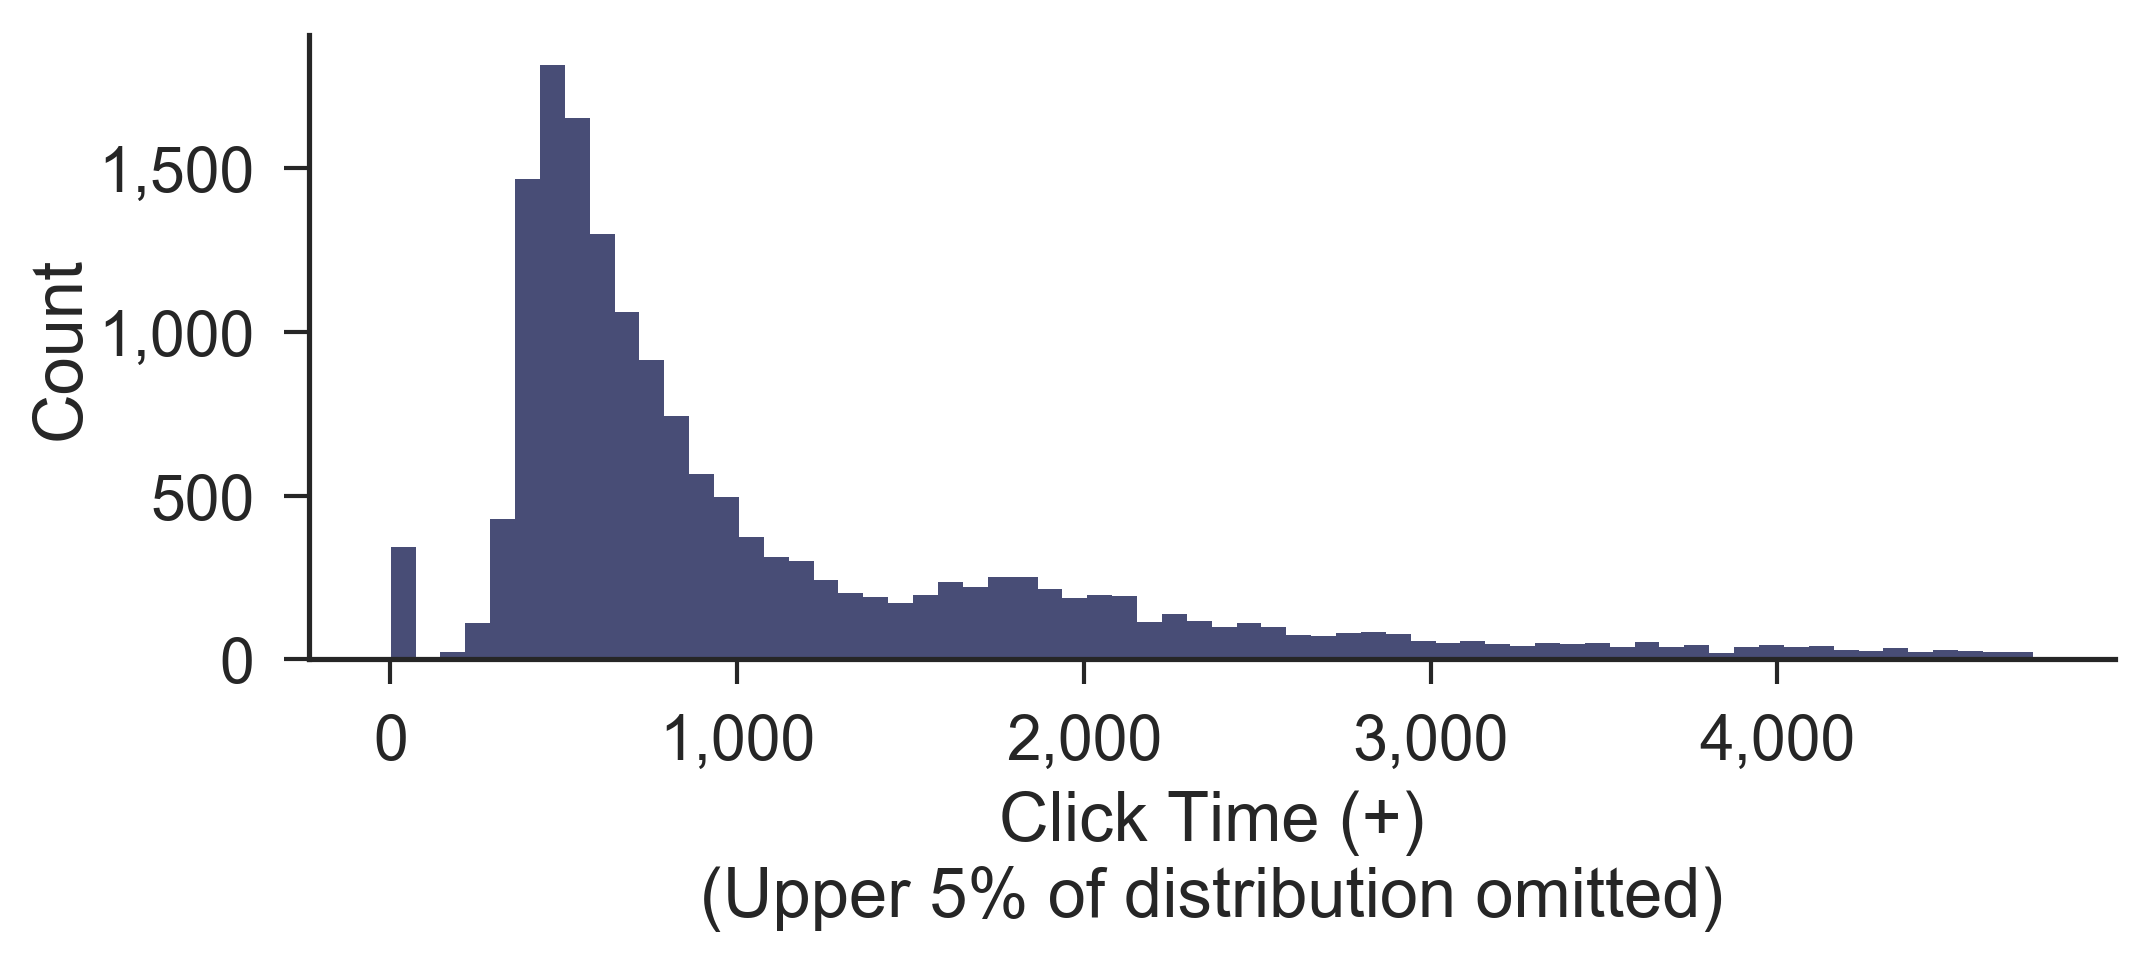
\includegraphics{/plot_clicktime_upper5omitted.png}

    \begin{Verbatim}[commandchars=\\\{\}]
{\color{incolor}In [{\color{incolor}3}]:} \PY{n}{rho} \PY{o}{=} \PY{n}{df}\PY{p}{[}\PY{p}{[}\PY{l+s+s1}{\PYZsq{}}\PY{l+s+s1}{Click Time (+)}\PY{l+s+s1}{\PYZsq{}}\PY{p}{,} \PY{l+s+s1}{\PYZsq{}}\PY{l+s+s1}{Render Time (+)}\PY{l+s+s1}{\PYZsq{}}\PY{p}{]}\PY{p}{]}\PY{o}{.}\PY{n}{corr}\PY{p}{(}\PY{n}{method}\PY{o}{=}\PY{l+s+s1}{\PYZsq{}}\PY{l+s+s1}{spearman}\PY{l+s+s1}{\PYZsq{}}\PY{p}{)}
        \PY{n}{NUM\PYZus{}BINS} \PY{o}{=} \PY{l+m+mi}{12}
        \PY{n}{figh}\PY{p}{,} \PY{p}{(}\PY{n}{ax1}\PY{p}{,} \PY{n}{ax2}\PY{p}{)} \PY{o}{=} \PY{n}{plt}\PY{o}{.}\PY{n}{subplots}\PY{p}{(}\PY{l+m+mi}{1}\PY{p}{,} \PY{l+m+mi}{2}\PY{p}{,} \PY{n}{figsize}\PY{o}{=}\PY{p}{(}\PY{l+m+mi}{12}\PY{p}{,} \PY{l+m+mi}{6}\PY{p}{)}\PY{p}{)}\PY{p}{;}
        \PY{n}{sns}\PY{o}{.}\PY{n}{regplot}\PY{p}{(}\PY{n}{df}\PY{p}{[}\PY{l+s+s1}{\PYZsq{}}\PY{l+s+s1}{Render Time (+)}\PY{l+s+s1}{\PYZsq{}}\PY{p}{]}\PY{p}{,} \PY{n}{df}\PY{p}{[}\PY{l+s+s1}{\PYZsq{}}\PY{l+s+s1}{Click Time (+)}\PY{l+s+s1}{\PYZsq{}}\PY{p}{]}\PY{p}{,} \PY{n}{ax}\PY{o}{=}\PY{n}{ax1}\PY{p}{,} \PY{n}{fit\PYZus{}reg}\PY{o}{=}\PY{k+kc}{False}\PY{p}{)}\PY{p}{;}
        \PY{n}{ax1}\PY{o}{.}\PY{n}{set\PYZus{}title}\PY{p}{(}\PY{l+s+s1}{\PYZsq{}}\PY{l+s+s1}{rank correlation = }\PY{l+s+si}{\PYZob{}:.2f\PYZcb{}}\PY{l+s+s1}{\PYZsq{}}\PY{o}{.}\PY{n}{format}\PY{p}{(}\PY{n}{rho}\PY{o}{.}\PY{n}{iloc}\PY{p}{[}\PY{l+m+mi}{0}\PY{p}{,}\PY{o}{\PYZhy{}}\PY{l+m+mi}{1}\PY{p}{]}\PY{p}{)}\PY{p}{)}\PY{p}{;}
        \PY{n}{ax2}\PY{o}{.}\PY{n}{set\PYZus{}ylabel}\PY{p}{(}\PY{l+s+s1}{\PYZsq{}}\PY{l+s+s1}{Click Time}\PY{l+s+s1}{\PYZsq{}}\PY{p}{)}\PY{p}{;} \PY{n}{ax2}\PY{o}{.}\PY{n}{set\PYZus{}xlabel}\PY{p}{(}\PY{l+s+s1}{\PYZsq{}}\PY{l+s+s1}{Render Time}\PY{l+s+s1}{\PYZsq{}}\PY{p}{)}\PY{p}{;}
        \PY{n}{sns}\PY{o}{.}\PY{n}{regplot}\PY{p}{(}\PY{n}{df}\PY{p}{[}\PY{l+s+s1}{\PYZsq{}}\PY{l+s+s1}{Render Time (+)}\PY{l+s+s1}{\PYZsq{}}\PY{p}{]}\PY{p}{,} \PY{n}{df}\PY{p}{[}\PY{l+s+s1}{\PYZsq{}}\PY{l+s+s1}{Click Time (+)}\PY{l+s+s1}{\PYZsq{}}\PY{p}{]}\PY{p}{,} \PY{n}{ax}\PY{o}{=}\PY{n}{ax2}\PY{p}{,} \PY{n}{x\PYZus{}bins}\PY{o}{=}\PY{n}{NUM\PYZus{}BINS}\PY{p}{,} \PY{n}{fit\PYZus{}reg}\PY{o}{=}\PY{k+kc}{False}\PY{p}{)}\PY{p}{;}
        \PY{n}{ax2}\PY{o}{.}\PY{n}{set\PYZus{}title}\PY{p}{(}\PY{l+s+s1}{\PYZsq{}}\PY{l+s+si}{\PYZob{}:d\PYZcb{}}\PY{l+s+s1}{ equally\PYZhy{}sized bins}\PY{l+s+s1}{\PYZsq{}}\PY{o}{.}\PY{n}{format}\PY{p}{(}\PY{n}{NUM\PYZus{}BINS}\PY{p}{)}\PY{p}{)}\PY{p}{;}
        \PY{n}{ax2}\PY{o}{.}\PY{n}{set\PYZus{}ylabel}\PY{p}{(}\PY{l+s+s1}{\PYZsq{}}\PY{l+s+s1}{Mean Click Time}\PY{l+s+s1}{\PYZsq{}}\PY{p}{)}\PY{p}{;} \PY{n}{ax2}\PY{o}{.}\PY{n}{set\PYZus{}xlabel}\PY{p}{(}\PY{l+s+s1}{\PYZsq{}}\PY{l+s+s1}{Render Time (Bin Mininum)}\PY{l+s+s1}{\PYZsq{}}\PY{p}{)}\PY{p}{;}
        \PY{n}{format\PYZus{}yticks}\PY{p}{(}\PY{n}{ax1}\PY{p}{)}\PY{p}{;} \PY{n}{format\PYZus{}yticks}\PY{p}{(}\PY{n}{ax2}\PY{p}{)}\PY{p}{;} \PY{n}{format\PYZus{}xticks}\PY{p}{(}\PY{n}{ax1}\PY{p}{)}\PY{p}{;}
        \PY{n}{figh}\PY{o}{.}\PY{n}{tight\PYZus{}layout}\PY{p}{(}\PY{p}{)}\PY{p}{;}
        \PY{n}{save\PYZus{}plot}\PY{p}{(}\PY{n}{figh}\PY{o}{=}\PY{n}{figh}\PY{p}{,} \PY{n}{outname}\PY{o}{=}\PY{l+s+s1}{\PYZsq{}}\PY{l+s+s1}{plot\PYZus{}clickxrender.png}\PY{l+s+s1}{\PYZsq{}}\PY{p}{)}\PY{p}{;}
\end{Verbatim}


    \begin{Verbatim}[commandchars=\\\{\}]

FIGURE SAVED TO: plot\_clickxrender.png

    \end{Verbatim}

    \hypertarget{the-relationship-between-click-time-and-render-time}{%
\subsection{The relationship between Click time and Render
time}\label{the-relationship-between-click-time-and-render-time}}

\begin{itemize}
\tightlist
\item
  Left pane is a scatter plot of the raw, positive-valued Click and
  Render times, which showed a moderately positive rank-order
  correlation
\item
  Right pane plots the average Click times for 12 equally-sized Render
  time bins to better visualize this positive correlation
\end{itemize}

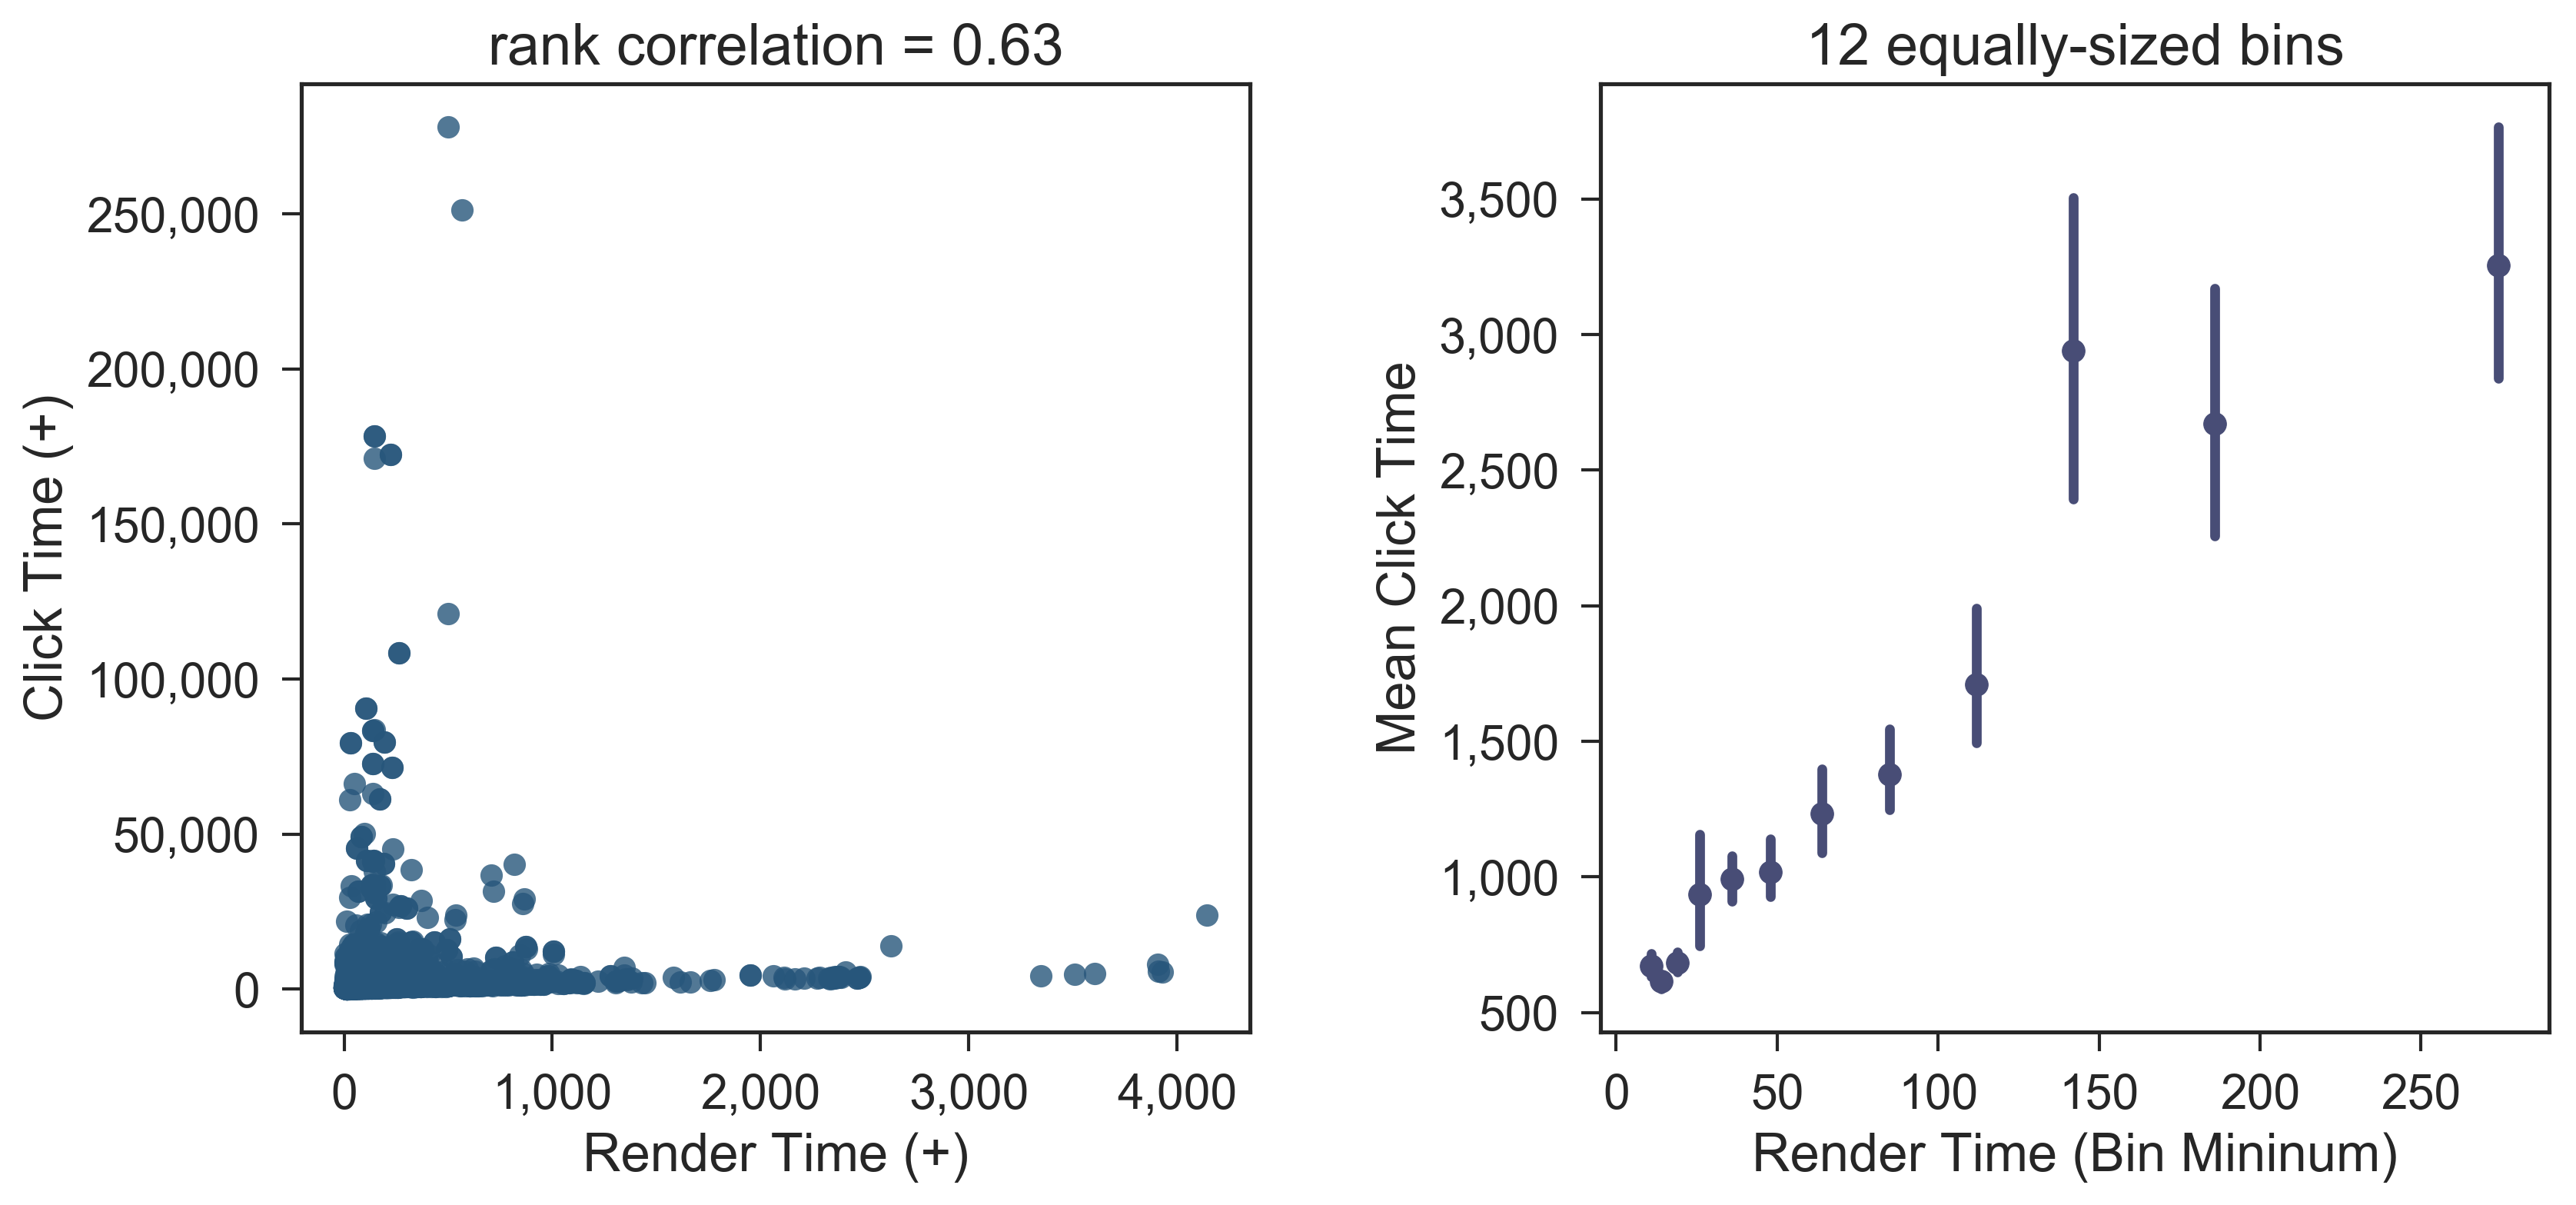
\includegraphics{/plot_clickxrender.png}

    \hypertarget{combinations-of-server-and-domain-that-have-the-biggest-issues-with-clicks-that-take-a-long-time-i.e.big-clicks}{%
\subsection{Combinations of Server and Domain that have the biggest
issues with clicks that take a long time (i.e.~Big
Clicks)}\label{combinations-of-server-and-domain-that-have-the-biggest-issues-with-clicks-that-take-a-long-time-i.e.big-clicks}}

\begin{itemize}
\tightlist
\item
  table shows \emph{Mean}, \emph{Standard Deviation (SD)}, and
  \emph{Maximum} for the 10 Server-Domain combos with the highest mean
  click times
\item
  the top 4 combos are distinguished by time distributions with big
  means and big variances
\end{itemize}

\begin{longtable}[]{@{}llrrrr@{}}
\toprule
Server & Domain & \emph{N} & Mean & SD & Max\tabularnewline
\midrule
\endhead
\textbf{CoreProcesses} & \textbf{HCM} & 578 & 39113 & 460223 &
8830183\tabularnewline
\textbf{FunctionalSetup} & \textbf{Common} & 4605 & 30598 & 468640 &
15553165\tabularnewline
\textbf{CRMCommon} & \textbf{CRM} & 320 & 23773 & 401079 &
7175832\tabularnewline
\textbf{Payable} & \textbf{Financial} & 1401 & 17517 & 288432 &
9326914\tabularnewline
\textbf{HelpPortal} & \textbf{Common} & 24 & 10977 & 41673 &
205250\tabularnewline
\textbf{SCMCommon} & \textbf{SCM} & 45 & 4189 & 13660 &
71375\tabularnewline
\textbf{HomePage} & \textbf{Common} & 8709 & 3792 & 108275 &
9095226\tabularnewline
\textbf{Procurement} & \textbf{Procurement} & 46 & 3413 & 11667 &
79476\tabularnewline
\textbf{ContractManagement} & \textbf{CRM} & 7 & 3214 & 3812 &
11173\tabularnewline
\textbf{GeneralLedger} & \textbf{Financial} & 284 & 2270 & 7188 &
116897\tabularnewline
\bottomrule
\end{longtable}

    \begin{Verbatim}[commandchars=\\\{\}]
{\color{incolor}In [{\color{incolor}18}]:} \PY{c+c1}{\PYZsh{} df.dropna(subset=[\PYZsq{}Click Time (+)\PYZsq{}], inplace=True)}
         \PY{n}{big\PYZus{}click\PYZus{}cutoffs} \PY{o}{=} \PY{p}{[}\PY{l+m+mi}{4000}\PY{p}{,} \PY{l+m+mi}{8000}\PY{p}{,} \PY{l+m+mi}{12000}\PY{p}{]}
         \PY{n}{name} \PY{o}{=} \PY{n}{big\PYZus{}click\PYZus{}cutoffs}\PY{o}{.}\PY{n}{copy}\PY{p}{(}\PY{p}{)}
         \PY{k}{for} \PY{n}{idx}\PY{p}{,}\PY{n}{c} \PY{o+ow}{in} \PY{n+nb}{enumerate}\PY{p}{(}\PY{n}{big\PYZus{}click\PYZus{}cutoffs}\PY{p}{)}\PY{p}{:}
             \PY{n}{name}\PY{p}{[}\PY{n}{idx}\PY{p}{]} \PY{o}{=} \PY{l+s+s1}{\PYZsq{}}\PY{l+s+si}{\PYZob{}:d\PYZcb{}}\PY{l+s+s1}{+ Clicks}\PY{l+s+s1}{\PYZsq{}}\PY{o}{.}\PY{n}{format}\PY{p}{(}\PY{n}{c}\PY{p}{)}
             \PY{n}{df}\PY{p}{[}\PY{n}{name}\PY{p}{[}\PY{n}{idx}\PY{p}{]}\PY{p}{]} \PY{o}{=} \PY{n}{df}\PY{p}{[}\PY{l+s+s1}{\PYZsq{}}\PY{l+s+s1}{Click Time (+)}\PY{l+s+s1}{\PYZsq{}}\PY{p}{]} \PY{o}{\PYZgt{}}\PY{o}{=} \PY{n}{c}
\end{Verbatim}


    \begin{Verbatim}[commandchars=\\\{\}]
{\color{incolor}In [{\color{incolor}19}]:} \PY{n}{pt} \PY{o}{=} \PY{n}{df}\PY{o}{.}\PY{n}{pivot\PYZus{}table}\PY{p}{(}\PY{n}{values}\PY{o}{=}\PY{l+s+s1}{\PYZsq{}}\PY{l+s+s1}{Click Time (+)}\PY{l+s+s1}{\PYZsq{}}\PY{p}{,} \PY{n}{index}\PY{o}{=}\PY{p}{[}\PY{l+s+s1}{\PYZsq{}}\PY{l+s+s1}{Server}\PY{l+s+s1}{\PYZsq{}}\PY{p}{,} \PY{l+s+s1}{\PYZsq{}}\PY{l+s+s1}{Domain}\PY{l+s+s1}{\PYZsq{}}\PY{p}{]}\PY{p}{,} \PY{n}{dropna}\PY{o}{=}\PY{k+kc}{True}\PY{p}{,} \PY{n}{margins}\PY{o}{=}\PY{k+kc}{False}\PY{p}{,} \PY{n}{aggfunc}\PY{o}{=}\PY{p}{[}\PY{l+s+s1}{\PYZsq{}}\PY{l+s+s1}{count}\PY{l+s+s1}{\PYZsq{}}\PY{p}{,} \PY{l+s+s1}{\PYZsq{}}\PY{l+s+s1}{mean}\PY{l+s+s1}{\PYZsq{}}\PY{p}{,} \PY{l+s+s1}{\PYZsq{}}\PY{l+s+s1}{median}\PY{l+s+s1}{\PYZsq{}}\PY{p}{,} \PY{l+s+s1}{\PYZsq{}}\PY{l+s+s1}{std}\PY{l+s+s1}{\PYZsq{}}\PY{p}{,} \PY{l+s+s1}{\PYZsq{}}\PY{l+s+s1}{max}\PY{l+s+s1}{\PYZsq{}}\PY{p}{]}\PY{p}{)}
         \PY{n}{pt}\PY{o}{.}\PY{n}{columns} \PY{o}{=} \PY{p}{[}\PY{l+s+s1}{\PYZsq{}}\PY{l+s+s1}{Count}\PY{l+s+s1}{\PYZsq{}}\PY{p}{,} \PY{l+s+s1}{\PYZsq{}}\PY{l+s+s1}{Mean}\PY{l+s+s1}{\PYZsq{}}\PY{p}{,} \PY{l+s+s1}{\PYZsq{}}\PY{l+s+s1}{Median}\PY{l+s+s1}{\PYZsq{}}\PY{p}{,} \PY{l+s+s1}{\PYZsq{}}\PY{l+s+s1}{SD}\PY{l+s+s1}{\PYZsq{}}\PY{p}{,} \PY{l+s+s1}{\PYZsq{}}\PY{l+s+s1}{Max}\PY{l+s+s1}{\PYZsq{}}\PY{p}{]}
         \PY{n}{pt} \PY{o}{=} \PY{n}{pt}\PY{o}{.}\PY{n}{sort\PYZus{}values}\PY{p}{(}\PY{n}{by}\PY{o}{=}\PY{l+s+s1}{\PYZsq{}}\PY{l+s+s1}{Mean}\PY{l+s+s1}{\PYZsq{}}\PY{p}{,} \PY{n}{ascending}\PY{o}{=}\PY{k+kc}{False}\PY{p}{)}\PY{o}{.}\PY{n}{apply}\PY{p}{(}\PY{k}{lambda} \PY{n}{x}\PY{p}{:} \PY{n}{x}\PY{o}{.}\PY{n}{astype}\PY{p}{(}\PY{n+nb}{int}\PY{p}{)}\PY{p}{)}\PY{o}{.}\PY{n}{head}\PY{p}{(}\PY{l+m+mi}{10}\PY{p}{)}
         \PY{n}{df2md}\PY{p}{(}\PY{n}{pt}\PY{p}{,} \PY{n}{ncol2bold}\PY{o}{=}\PY{l+m+mi}{2}\PY{p}{)}
\end{Verbatim}


    \begin{Verbatim}[commandchars=\\\{\}]
|        Server        |    Domain     |Count|Mean |Median|  SD  |  Max   |
|----------------------|---------------|----:|----:|-----:|-----:|-------:|
|**CoreProcesses**     |**HCM**        |  578|39113|  1045|460223| 8830183|
|**FunctionalSetup**   |**Common**     | 4605|30598|   993|468640|15553165|
|**CRMCommon**         |**CRM**        |  320|23773|   574|401079| 7175832|
|**Payable**           |**Financial**  | 1401|17517|   931|288432| 9326914|
|**HelpPortal**        |**Common**     |   24|10977|   517| 41673|  205250|
|**SCMCommon**         |**SCM**        |   45| 4189|   984| 13660|   71375|
|**HomePage**          |**Common**     | 8709| 3792|   539|108275| 9095226|
|**Procurement**       |**Procurement**|   46| 3413|   951| 11667|   79476|
|**ContractManagement**|**CRM**        |    7| 3214|  1564|  3812|   11173|
|**GeneralLedger**     |**Financial**  |  284| 2270|  1193|  7188|  116897|


    \end{Verbatim}

    \begin{Verbatim}[commandchars=\\\{\}]
{\color{incolor}In [{\color{incolor}24}]:} \PY{n}{g} \PY{o}{=} \PY{n}{df}\PY{o}{.}\PY{n}{dropna}\PY{p}{(}\PY{p}{)}\PY{o}{.}\PY{n}{groupby}\PY{p}{(}\PY{p}{[}\PY{l+s+s1}{\PYZsq{}}\PY{l+s+s1}{Server}\PY{l+s+s1}{\PYZsq{}}\PY{p}{,} \PY{l+s+s1}{\PYZsq{}}\PY{l+s+s1}{Domain}\PY{l+s+s1}{\PYZsq{}}\PY{p}{]}\PY{p}{)}\PY{p}{[}\PY{n}{name}\PY{p}{]}
         \PY{n}{p} \PY{o}{=} \PY{l+m+mi}{100}\PY{o}{*}\PY{p}{(}\PY{n}{g}\PY{o}{.}\PY{n}{sum}\PY{p}{(}\PY{p}{)} \PY{o}{/} \PY{n}{g}\PY{o}{.}\PY{n}{count}\PY{p}{(}\PY{p}{)}\PY{p}{)}\PY{o}{.}\PY{n}{dropna}\PY{p}{(}\PY{p}{)}\PY{o}{.}\PY{n}{sort\PYZus{}values}\PY{p}{(}\PY{n}{by}\PY{o}{=}\PY{n}{name}\PY{p}{[}\PY{l+m+mi}{0}\PY{p}{]}\PY{p}{,} \PY{n}{ascending}\PY{o}{=}\PY{k+kc}{False}\PY{p}{)}\PY{o}{.}\PY{n}{head}\PY{p}{(}\PY{l+m+mi}{10}\PY{p}{)}
         \PY{n}{df2md}\PY{p}{(}\PY{n}{p}\PY{p}{,} \PY{n}{ncol2bold}\PY{o}{=}\PY{l+m+mi}{2}\PY{p}{)}
\end{Verbatim}


    \begin{Verbatim}[commandchars=\\\{\}]
|        Server        |    Domain     |4000+ Clicks|8000+ Clicks|12000+ Clicks|
|----------------------|---------------|-----------:|-----------:|------------:|
|**ContractManagement**|**CRM**        |       28.57|       14.29|         0.00|
|**CoreProcesses**     |**HCM**        |       11.46|        7.05|         4.59|
|**Procurement**       |**Procurement**|       10.87|        6.52|         2.17|
|**SCMCommon**         |**SCM**        |        8.89|        6.67|         4.44|
|**FunctionalSetup**   |**Common**     |        7.93|        2.85|         1.71|
|**Payable**           |**Financial**  |        7.42|        2.33|         1.02|
|**FinancialCommon**   |**Financial**  |        7.06|        3.45|         2.04|
|**GeneralLedger**     |**Financial**  |        7.01|        1.11|         1.11|
|**CoreSetup**         |**HCM**        |        6.81|        3.19|         2.23|
|**HelpPortal**        |**Common**     |        5.00|        5.00|         5.00|


    \end{Verbatim}

    \hypertarget{other-useful-insights}{%
\section{Other useful insights}\label{other-useful-insights}}

    \hypertarget{non-positive-click-times-evenly-distributed-across-server-domains-combos}{%
\subsection{Non-Positive Click Times: evenly distributed across
Server-Domains
combos?}\label{non-positive-click-times-evenly-distributed-across-server-domains-combos}}

\begin{itemize}
\tightlist
\item
  counts of \emph{Negative}, \emph{Positive}, and \emph{Zero} values
  observed for the 10 Server-Domain combos with the highest number of
  negative values
\item
  the \textbf{HomePage-Common} combo has an exceptionally high frequency
  of non-positive values and deserves special attention
\end{itemize}

\begin{longtable}[]{@{}llrrr@{}}
\toprule
Server & Domain & \emph{N}Negative & \emph{N}Positive &
\emph{N}Zero\tabularnewline
\midrule
\endhead
\textbf{HomePage} & \textbf{Common} & 13470 & 8709 & 4757\tabularnewline
\textbf{FunctionalSetup} & \textbf{Common} & 4604 & 4605 &
1\tabularnewline
\textbf{Payable} & \textbf{Financial} & 1408 & 1401 & 8\tabularnewline
\textbf{CoreSetup} & \textbf{HCM} & 944 & 942 & 0\tabularnewline
\textbf{FinancialCommon} & \textbf{Financial} & 644 & 639 &
0\tabularnewline
\textbf{CoreProcesses} & \textbf{HCM} & 585 & 578 & 7\tabularnewline
\textbf{CRMCommon} & \textbf{CRM} & 325 & 320 & 5\tabularnewline
\textbf{GeneralLedger} & \textbf{Financial} & 253 & 284 &
2\tabularnewline
\textbf{Procurement} & \textbf{Procurement} & 46 & 46 & 0\tabularnewline
\textbf{SCMCommon} & \textbf{SCM} & 45 & 45 & 0\tabularnewline
\bottomrule
\end{longtable}

    \begin{Verbatim}[commandchars=\\\{\}]
{\color{incolor}In [{\color{incolor}26}]:} \PY{n}{ct} \PY{o}{=} \PY{n}{pd}\PY{o}{.}\PY{n}{crosstab}\PY{p}{(}\PY{n}{df}\PY{p}{[}\PY{l+s+s1}{\PYZsq{}}\PY{l+s+s1}{Click Time Sign}\PY{l+s+s1}{\PYZsq{}}\PY{p}{]}\PY{p}{,} \PY{p}{[}\PY{n}{df}\PY{o}{.}\PY{n}{Server}\PY{p}{,} \PY{n}{df}\PY{o}{.}\PY{n}{Domain}\PY{p}{]}\PY{p}{)}\PY{o}{.}\PY{n}{transpose}\PY{p}{(}\PY{p}{)}\PY{o}{.}\PY{n}{sort\PYZus{}values}\PY{p}{(}\PY{n}{by}\PY{o}{=}\PY{l+s+s1}{\PYZsq{}}\PY{l+s+s1}{Negative}\PY{l+s+s1}{\PYZsq{}}\PY{p}{,} \PY{n}{ascending}\PY{o}{=}\PY{k+kc}{False}\PY{p}{)}\PY{o}{.}\PY{n}{head}\PY{p}{(}\PY{l+m+mi}{10}\PY{p}{)}\PY{p}{;}
         \PY{n}{ct}\PY{o}{.}\PY{n}{columns} \PY{o}{=} \PY{p}{[}\PY{l+s+s1}{\PYZsq{}}\PY{l+s+s1}{*N*\PYZlt{}br\PYZgt{}Negative}\PY{l+s+s1}{\PYZsq{}}\PY{p}{,} \PY{l+s+s1}{\PYZsq{}}\PY{l+s+s1}{*N*\PYZlt{}br\PYZgt{}Positive}\PY{l+s+s1}{\PYZsq{}}\PY{p}{,} \PY{l+s+s1}{\PYZsq{}}\PY{l+s+s1}{*N*\PYZlt{}br\PYZgt{}Zero}\PY{l+s+s1}{\PYZsq{}}\PY{p}{]}
         \PY{n}{df2md}\PY{p}{(}\PY{n}{ct}\PY{p}{,} \PY{n}{ncol2bold}\PY{o}{=}\PY{l+m+mi}{2}\PY{p}{)}
\end{Verbatim}


    \begin{Verbatim}[commandchars=\\\{\}]
|      Server       |    Domain     |*N*<br>Negative|*N*<br>Positive|*N*<br>Zero|
|-------------------|---------------|--------------:|--------------:|----------:|
|**HomePage**       |**Common**     |          13470|           8709|       4757|
|**FunctionalSetup**|**Common**     |           4604|           4605|          1|
|**Payable**        |**Financial**  |           1408|           1401|          8|
|**CoreSetup**      |**HCM**        |            944|            942|          0|
|**FinancialCommon**|**Financial**  |            644|            639|          0|
|**CoreProcesses**  |**HCM**        |            585|            578|          7|
|**CRMCommon**      |**CRM**        |            325|            320|          5|
|**GeneralLedger**  |**Financial**  |            253|            284|          2|
|**Procurement**    |**Procurement**|             46|             46|          0|
|**SCMCommon**      |**SCM**        |             45|             45|          0|


    \end{Verbatim}

    \hypertarget{which-combos-have-the-highest-percentage-of-big-clicks}{%
\subsection{\texorpdfstring{Which combos have the highest \% percentage
of \emph{Big
Clicks}?}{Which combos have the highest \% percentage of Big Clicks?}}\label{which-combos-have-the-highest-percentage-of-big-clicks}}

\begin{itemize}
\tightlist
\item
  table shows the top 10 combos logging the highest percentage of clicks
  greater than or equal to 4,000, 8,000, or 12,000
\end{itemize}

\begin{longtable}[]{@{}llrrr@{}}
\toprule
Server & Domain & 4000+ Clicks & 8000+ Clicks & 12000+
Clicks\tabularnewline
\midrule
\endhead
\textbf{ContractManagement} & \textbf{CRM} & 28.57 & 14.29 &
0.00\tabularnewline
\textbf{HelpPortal} & \textbf{Common} & 16.67 & 12.50 &
12.50\tabularnewline
\textbf{CoreProcesses} & \textbf{HCM} & 12.80 & 8.30 &
5.88\tabularnewline
\textbf{GeneralLedger} & \textbf{Financial} & 10.92 & 2.46 &
2.11\tabularnewline
\textbf{Procurement} & \textbf{Procurement} & 10.87 & 6.52 &
2.17\tabularnewline
\textbf{FunctionalSetup} & \textbf{Common} & 9.34 & 3.95 &
2.74\tabularnewline
\textbf{Payable} & \textbf{Financial} & 9.14 & 3.71 &
2.43\tabularnewline
\textbf{SCMCommon} & \textbf{SCM} & 8.89 & 6.67 & 4.44\tabularnewline
\textbf{FinancialCommon} & \textbf{Financial} & 7.36 & 3.76 &
2.19\tabularnewline
\textbf{CoreSetup} & \textbf{HCM} & 6.90 & 3.29 & 2.34\tabularnewline
\bottomrule
\end{longtable}


    % Add a bibliography block to the postdoc
    
    
    
    \end{document}
